
\section{Results}\notinsubfile{\label{sec:results}}
%\setcounter{page}{0}\pagenumbering{arabic}

\subsubsection{The model with no returns heterogeneity}

\par To solve and simulate the model, I follow the calibration scheme captured in table \ref{tab:calib1}.
\hypertarget{calibPY}{}
\begin{table}[ht]
  \centering
  \resizebox{0.7\textwidth}{!}{
    \begin{tabular}{cccc}
        \toprule
        Description & Parameter & Value & Source \\
        \midrule
        Time discount factor & $\beta$ & 0.99 & \cite{Den_Haan2010} \\
        CRRA & $\rho$ & 1 & \cite{Den_Haan2010} \\
        Capital share & $\alpha$ & 0.36 & \cite{Den_Haan2010} \\
        Depreciation rate & $\delta$ & 0.025 & \cite{Den_Haan2010} \\
        Time worked per employee & $\ell$ & 1/.09 & \cite{Den_Haan2010} \\
        Capital/output ratio & $\frac{K}{Y}$ & 10.26 & \cite{Den_Haan2010} \\
        Effective interest rate & $r - \delta$ & 0.01 & \cite{Den_Haan2010} \\
        Wage rate & $W$ & 2.37 & \cite{Den_Haan2010} \\
        Unempl. insurance payment & $\mu$ & 0.15 & \cite{Den_Haan2010} \\
        Probability of death & $D$ & 0.00625 & Yields 40-year working life \\
        Variance of $\log \theta_{t,i}$ & $\sigma^{2}_{\theta}$ & 0.010 x 4 & \begin{tabular}[t]{@{}p{5.5cm}@{}} \cite{Carroll1992}, \\ \cite{Carroll2015} \end{tabular} \\
        Variance of $\log \psi_{t,i}$ & $\sigma^{2}_{\psi}$ & 0.010 x 4/11 & \begin{tabular}[t]{@{}p{5.5cm}@{}} \cite{Carroll1992}, \\  \cite{Debacker2013},  \\ \cite{Carroll2015} \end{tabular} \\
        Unemployment rate & $\mho$ & 0.07 & Mean in \cite{Den_Haan2010} \\
        \bottomrule
    \end{tabular}
    }
    \caption{Parameter values (quarterly frequency) for the perpetual youth (infinite horizon) model.}
    \label{tab:calib1}
\end{table}

\unskip

\par The solution of the model with no heterogeneity in returns (the R-point model) is the one which finds the value for the rate of return $R$ which minimizes the distance between the simulated and empirical wealth shares at the 20th, 40th, 60th, and 80th percentiles. The empirical targets are computed using the 2004 SCF data on household wealth. The estimation procedure finds this optimal value to be $R = 1.0602$.

\subsubsection{Incorporating heterogeneous returns}

\par As noted above, recent studies by \cite{aflgdmlp20} and \cite{lblcps18} have not only estimated the rate of return on asset holdings but have also uncovered significant heterogeneity across households. With this in mind, the next estimation (the R-dist model) assumes the existence of multiple types of agents, each earning a distinct rate of return on their assets.

\par I follow closely the procedure outlined by \cite{cstw2017}. Specifically, I assume that different types of households have a time preference factor drawn from a uniform distribution on the interval $(\grave{R} - \nabla, \grave{R} + \nabla)$, where $\nabla$ represents the level of dispersion. Afterward, the model is simulated to estimate the values of both $\grave{R}$ and $\nabla$ so that the model matches the inequality in the wealth distribution. To achieve this, the following minimization problem is solved:

$$ \{\grave{R}, \nabla\} = \text{arg}\min_{R, \nabla} \bigg( \sum_{i=20, 40, 60, 80} (w_{i}(R, \nabla)-\omega_i )^{2} \bigg)^{\frac{1}{2}} $$

\par subject to the constraint that the aggregate capital-to-output ratio in this model matches the calibrated value $5$. This is towards the upper bound on plausibly calibrated values for the capital-to-output ratio, as much of the literature chooses values between $2$ and  $3$.

\par Note that $w_i$ and $\omega_i$ give the porportion of total aggregate net worth held by the top $i$ percent in the model and in the data, respectively.

\par The estimation procedure finds this optimal values of $R = 1.0212$ and $\nabla = 0.06728$. These parameter values pin down the estimated uniform distribution. In the model, I've chosen to discretize that distribution to 7 chosen points. The performance of the estimation of both the R-point and R-dist models, measured by their ability to match the SCF data, is compared in figure \ref{fig:PYUnif}.

\begin{figure}[h]
    \centering
    \begin{minipage}{0.48\textwidth}
        \centering
        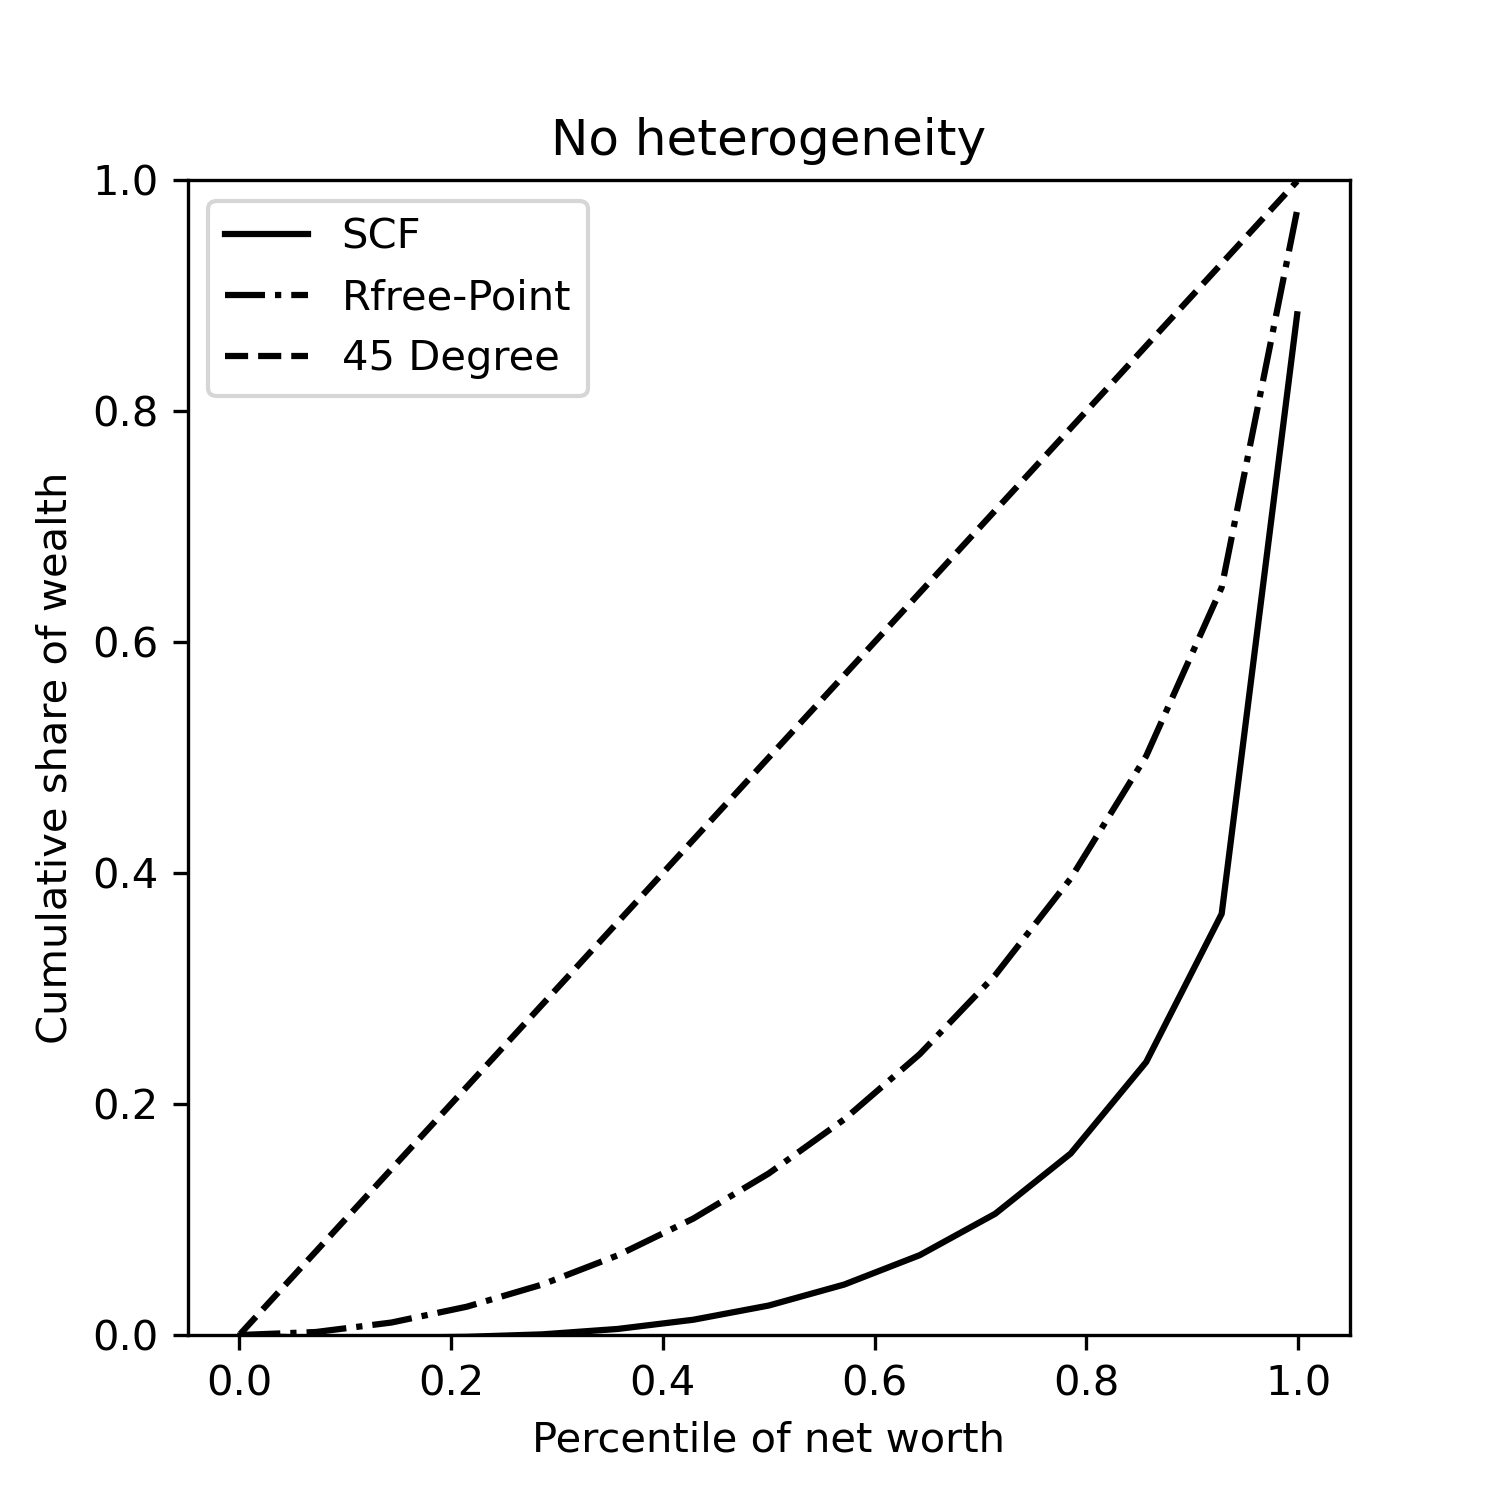
\includegraphics[width=\textwidth]{../Figures/PYrrPointNetWorthPlot.png}
    \end{minipage}
    \hfill
    \begin{minipage}{0.48\textwidth}
        \centering
        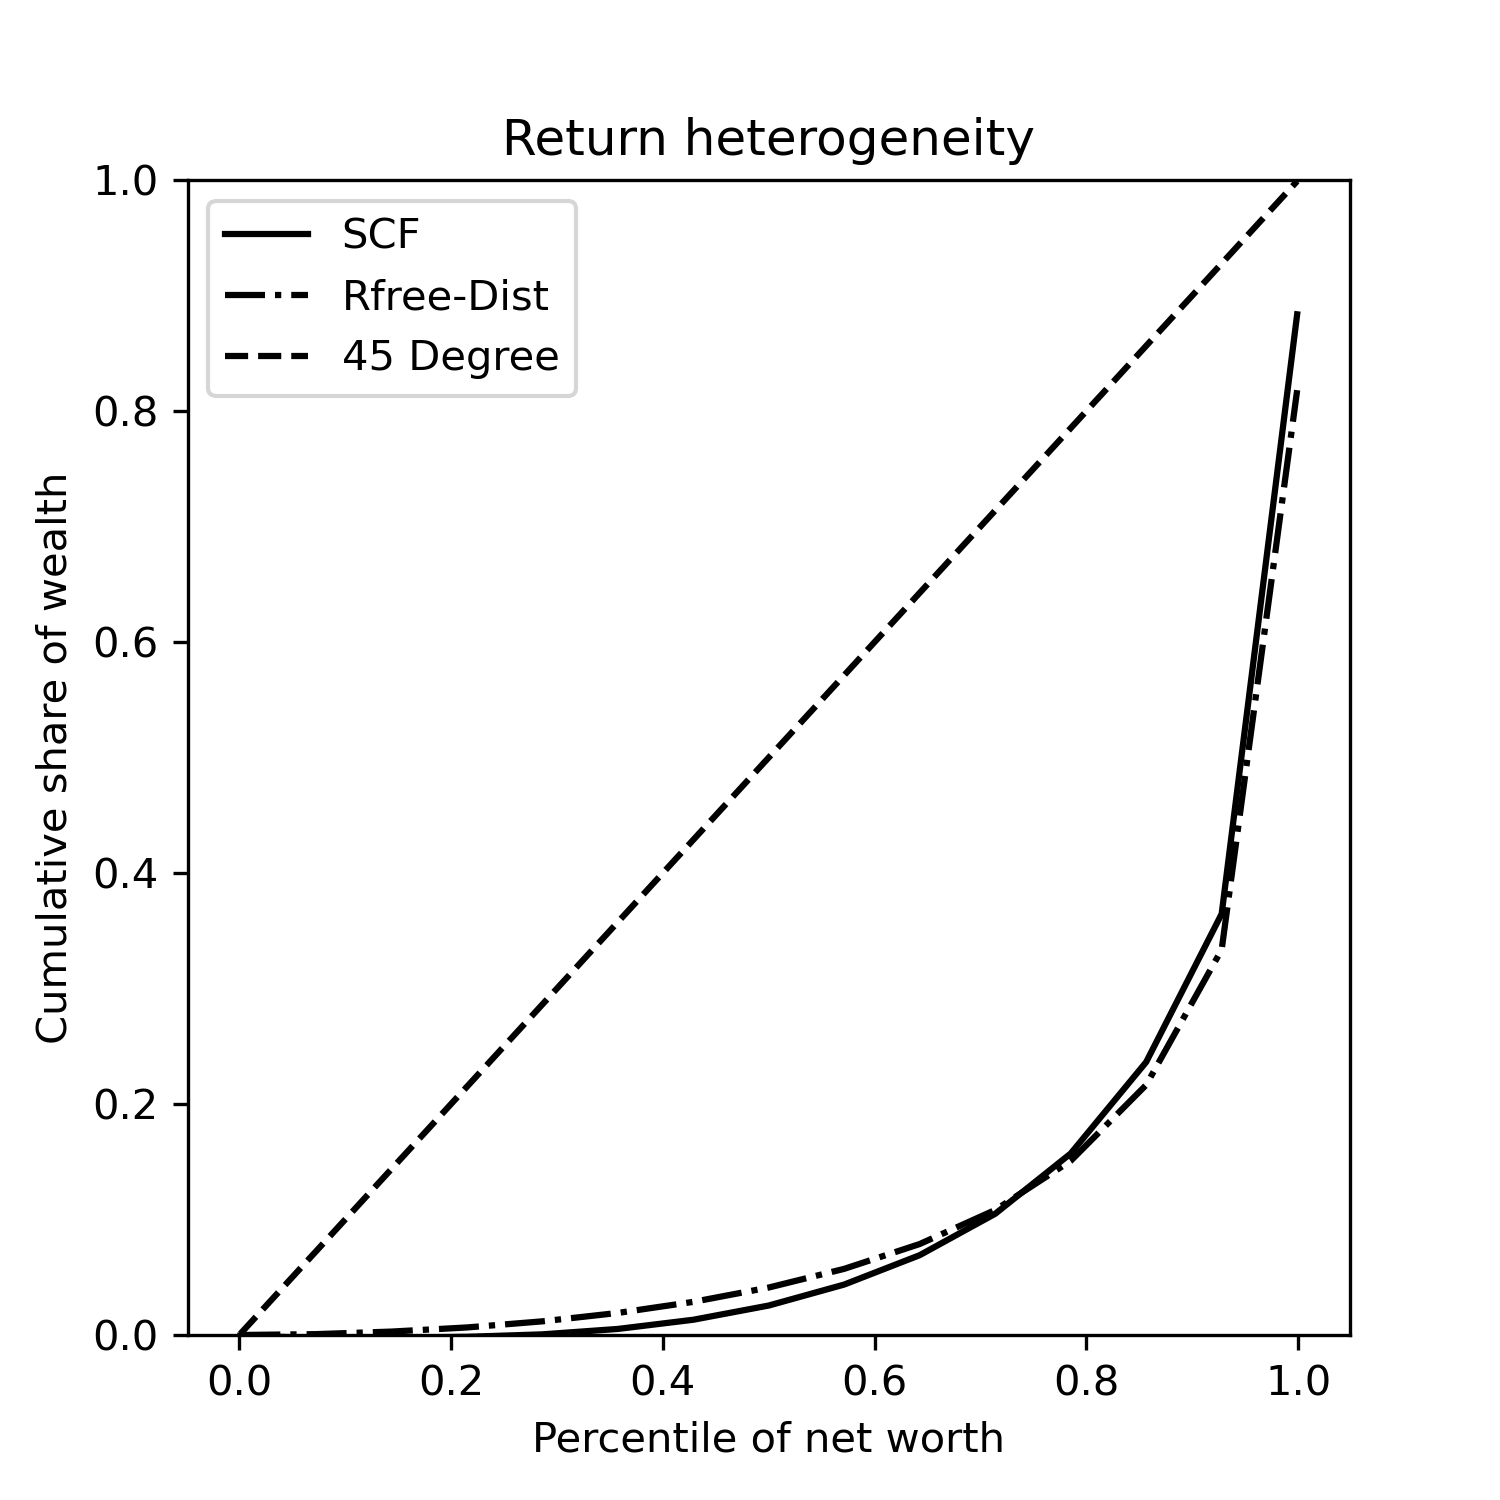
\includegraphics[width=\textwidth]{../Figures/PYrrDistNetWorthPlot.png}
    \end{minipage}
    \caption{Comparison of R-Point and R-Dist Models.}
    \label{fig:PYUnif} 
\end{figure}


\subsection{Incorporating life cycle dynamics into the model}

\par More realistic assumptions regarding the age and education level of households can have important implications for the income and mortality process of households. Here, I extend the model to incorporate these life cycle dynamics.

\par Households enter the economy at time $t$ aged 24 years old and are endowed with an education level $e \in \{D,HS,C\}$, and initial permanent income level $\textbf{p}_0$, and a capital stock $k_0$. The life cycle version of household income is given by:

$$ y_t = \xi_t \textbf{p}_t = (1 - \tau) \theta_t \textbf{p}_t, $$

where $\textbf{p}_t = \psi_t \bar{\psi}_{es} \textbf{p}_{t-1}$ and $\bar{\psi}_{es}$ captures the age-education-specific average growth factor. Households that have lived for $s$ periods have permanent shocks drawn from a lognormal distribution with mean $1$ and variance $\sigma^{2}_{\psi s}$ and transitory shocks drawn from a lognormal distribution with mean $\frac{1}{\cancel{\mho}}$ and variance $\sigma^{2}_{\theta s}$ with probability $\cancel{\mho} = (1-\mho)$ and $\mu$ with probability $\mho$.

\par The normalized version of the age-education-specific consumption-saving problem for households is given by

\begin{eqnarray*}
  v_{es}(m_t) &=& \max_{c_t} u(c_t(m_t)) + \beta \cancel{D}_{es} \mathbb{E}_{t}[\psi_{t+1}^{1-\rho}v_{es + 1}(m_{t+1})] \\
  &\text{s.t.}& \\
  a_t &=& m_t - c_t, \\
  k_{t+1} &=& \frac{a_t}{\psi_{t+1}}, \\
  m_{t+1} &=& (\daleth + r_t)k_{t+1} + \xi_{t+1}, \\
  a_t &\geq& 0.
\end{eqnarray*}

\par The additional parameters necessary to calibrate the life cycle version of the model are given in table \ref{tab:calib2}.

\hypertarget{calibLC}{}
\begin{table}[ht]
  \centering
  \resizebox{0.6\textwidth}{!}{
    \begin{tabular}{ccc}
        \toprule
        Description & Parameter & Value  \\
        \midrule
        Population growth rate & $N$ & 0.0025  \\
        Technological growth rate & $\Gamma$ & 0.0037  \\
        Rate of high school dropouts & $\theta_D $ & 0.11  \\
        Rate of high school graduates & $\theta_{HS} $ & 0.55  \\
        Rate of college graduates & $\theta_C $ & 0.34  \\
        Labor income tax rate & $\tau$ & 0.0942  \\
        \bottomrule
    \end{tabular}}
    \caption{Parameter values (annual frequency) for the lifecycle model.}
    \label{tab:calib2}
\end{table}

\unskip

\par The estimation procedure finds this optimal value to be $R = 1.0414$ for the R-point model in this setting. The estimation procedure for the R-dist model in the life cycle setting finds optimal values of $R = 1.0343$ and $\nabla =0.03557$. Notice the improved performance of the estimation in matching the data displayed in figure \ref{fig:LCUnif}.

\begin{figure}[h]
    \centering
    \begin{minipage}{0.48\textwidth}
        \centering
        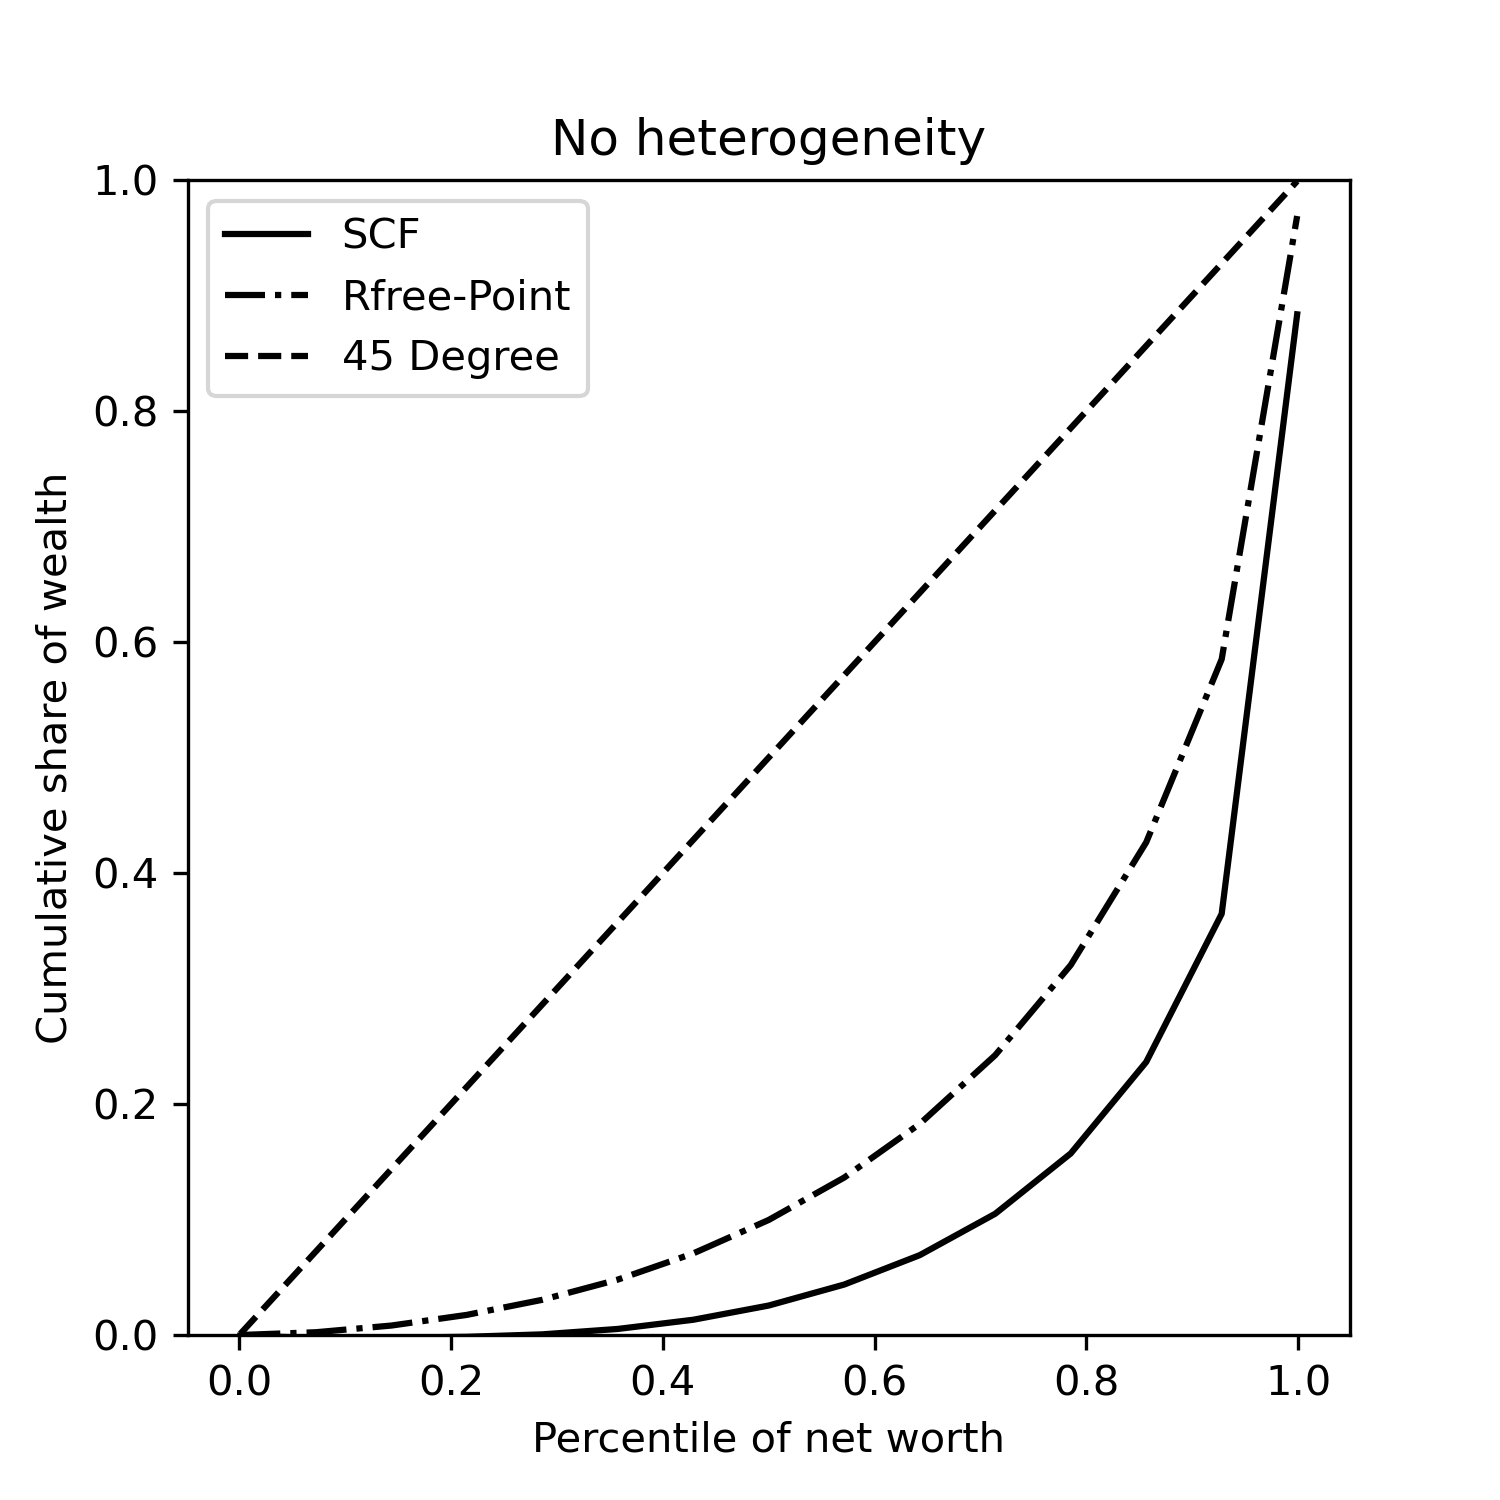
\includegraphics[width=\textwidth]{../Figures/LCrrPointNetWorthPlot.png}
    \end{minipage}
    \hfill
    \begin{minipage}{0.48\textwidth}
        \centering
        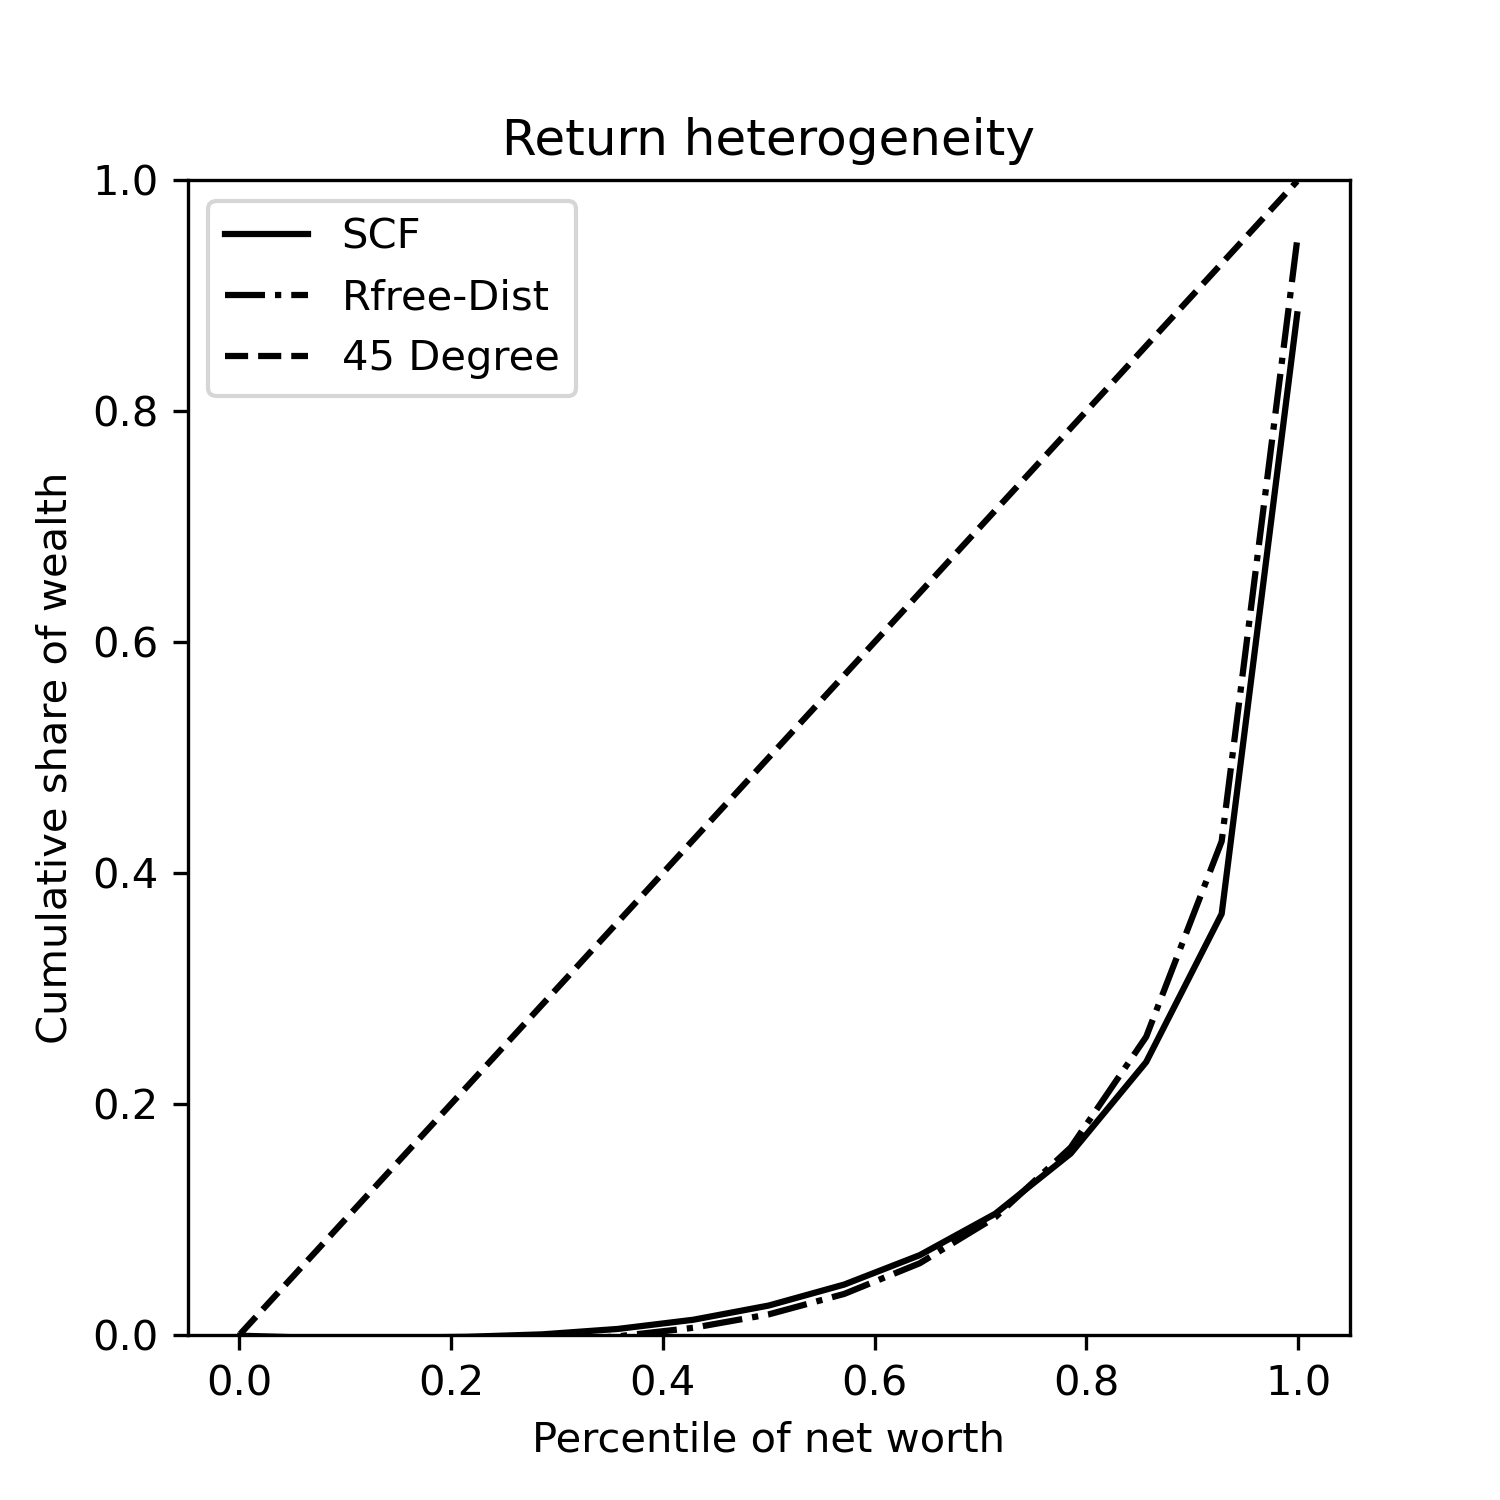
\includegraphics[width=\textwidth]{../Figures/LCrrDistNetWorthPlot.png}
    \end{minipage}
    \caption{Comparison of R-Point and R-Dist Models in the Life-Cycle Setting.}
    \label{fig:LCUnif} 
  \end{figure}

  \subsection{The implied distribution of bank heterogeneity}

  \par First, recall that we provided a simple model for the bank's decision problem, where profits depend only on the dispersion between the market interest rate $R^m$ and the offered deposit rate $R^d$ and the level of foreign deposits that the banks hold. Since I chose to model the demand for foreign deposits with an isoelastic demand function $S_i(R^d) = A_i (R_i^d)^{\varepsilon_i}$ , this implies that the \textit{elasticity of foreign deposits to the interest rate} is given by

  \begin{align}
    \varepsilon_i = \frac{\partial S_i(R^d)}{\partial R^d} \frac{R^d}{S_i(R^d)}
  \end{align}

  for each bank $i$. Thus, since I've estimated the distribution of returns which matches the wealth moements, I can use this feature of the model to back out an implied distribution of $\varepsilon$, which will describe how the banks differ in their sensitivities to foreign deposit outflows, ultimately affecting their optimal choice of the offered deposit rates. 

  \par To do this, I assume that the aggregate production function is Cobb-douglas, so that the marginal product of capital can be written as $\alpha \frac{Y}{K}$. With the calibrated values  $\delta = .025$, $\alpha = .36$, and the capital to output ratio $3$  matched by using the 2004 SCF, this setting has an effective interest rate of $R^m = 1.095$ which can be used as the market interest rate.

  \par Since the model with heterogeneity (i.e. the R-dist model) has 7 estimated points for the uniform distribution, the implied, estimated points for $\varepsilon$ can be uniquely pineed down by the expression $$\varepsilon_i = \frac{R_i^d}{R^m - R_i^d} .$$

  \par % are given by $[ 0.0423, 0.1731, 0.3414, 0.5661, 0.8812, 1.3551, 2.1482 ]$.

  \par Following the logic of the  elasticity of foreign deposits to the interest rate in the work by \cite{Sarkisyan2021}, globally integrated banks would face larger foregin deposit outflows when the offered deposit rate is significantly further than the market interest rate. These would be precisely the banks with higher elasticities -- in my descritized model with 7 points, this would suggest that the last two banks may be interpreted as globally integrated. The individuals \say{stuck} with banking at this institution (since I assume that households cannot switch banks) would be relatively better of than their counterparts, as they will receive a higher offered deposit rate.  
 

\subsection{Untargeted moments}

\par It is well-documented in the literature on heterogeneous agent modeling that, adding a source of (ex-ante) heterogeneous beyond the addition of labor income uncertainty to the representative agent framework will allow the simulated distribution of wealth to match moments of the empirical wealth distribution particularly well. So, although it is useful to see that the model with heterogeneous returns does a good job of matching the given lorenz targets, we need another way to assess the model's performance.

\par For this reason, I include age-dependent wealth moments from the same wave of the SCF to serve as untargeted moments~\ref{fig:EmpLorenzTar}. These can be found in the following table~\ref{fig:EmpLorenzTar}.

\begin{figure}[h]
\centering
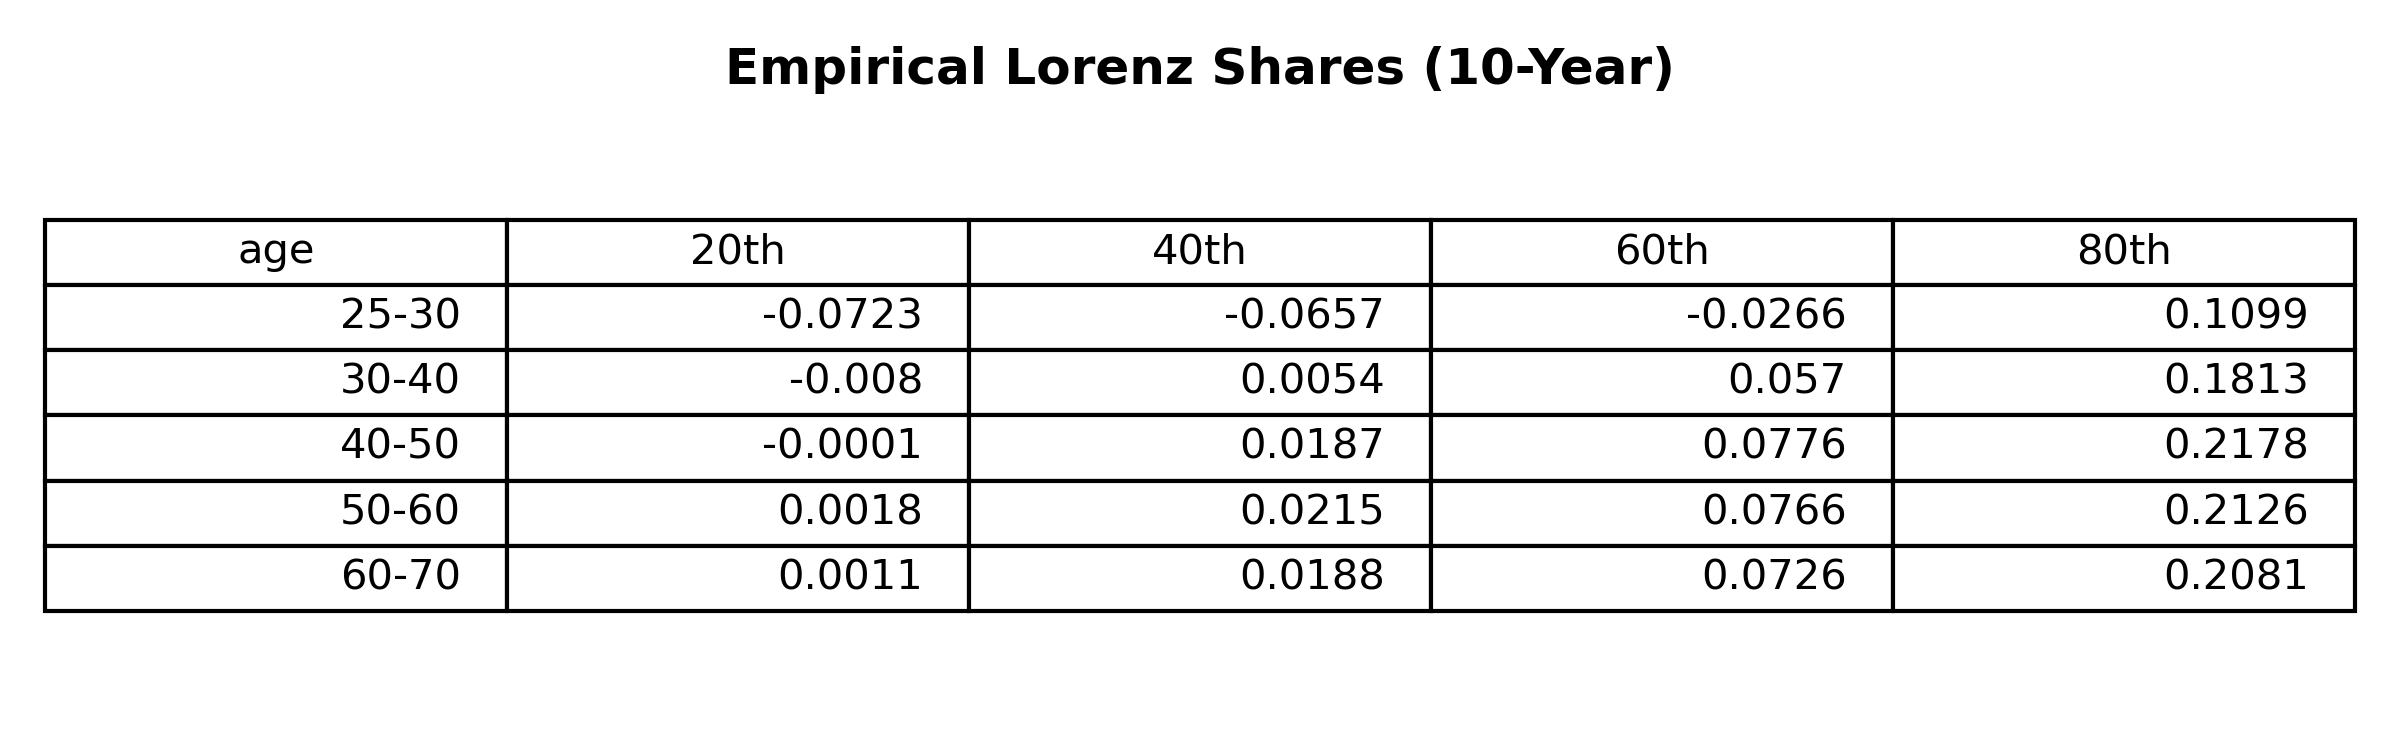
\includegraphics[width=0.8\textwidth]{Tables/Emp_Lorenz_10yr_LCrrDistNetWorth.png}
\caption{Empirical Lorenz Curve Targets from the 2004 SCF.}
\label{fig:EmpLorenzTar}
\end{figure}

\par The next two tables present the simulated version of the untargeted moments for the model without heterogeneity~\ref{fig:SimLorenzTarPoint}, and then with heterogeneity~\ref{fig:SimLorenzTarDist}. As you can see from the tables~\ref{fig:SimLorenzTarPoint} and~\ref{fig:SimLorenzTarDist} below, the age-dependent Lorenz targets that arise from the model again fit the data much better when returns heterogeneity is present versus when it is absent.

\begin{figure}[htbp]
\centering
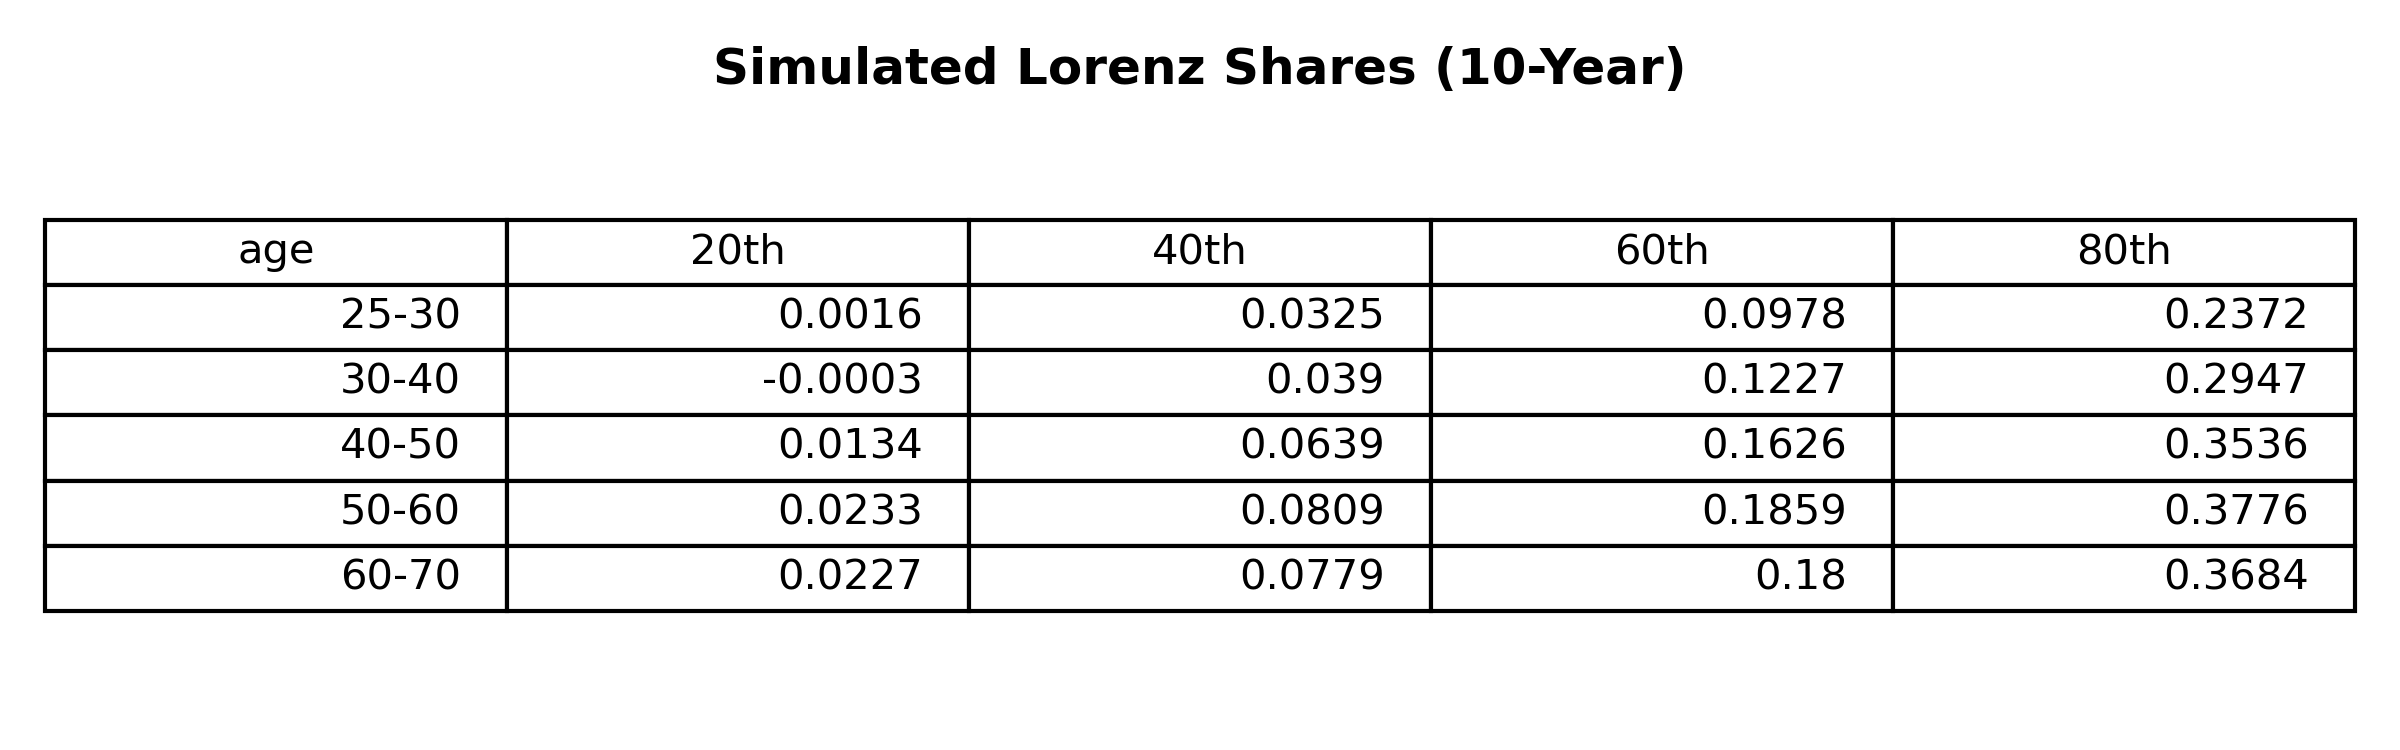
\includegraphics[width=0.8\textwidth]{Tables/Sim_Lorenz_10yr_LCrrPointNetWorth.png}
\caption{Simulated Untargeted Moments without Heterogeneity (R-point).}
\label{fig:SimLorenzTarPoint}
\end{figure}

\begin{figure}[htbp]
\centering
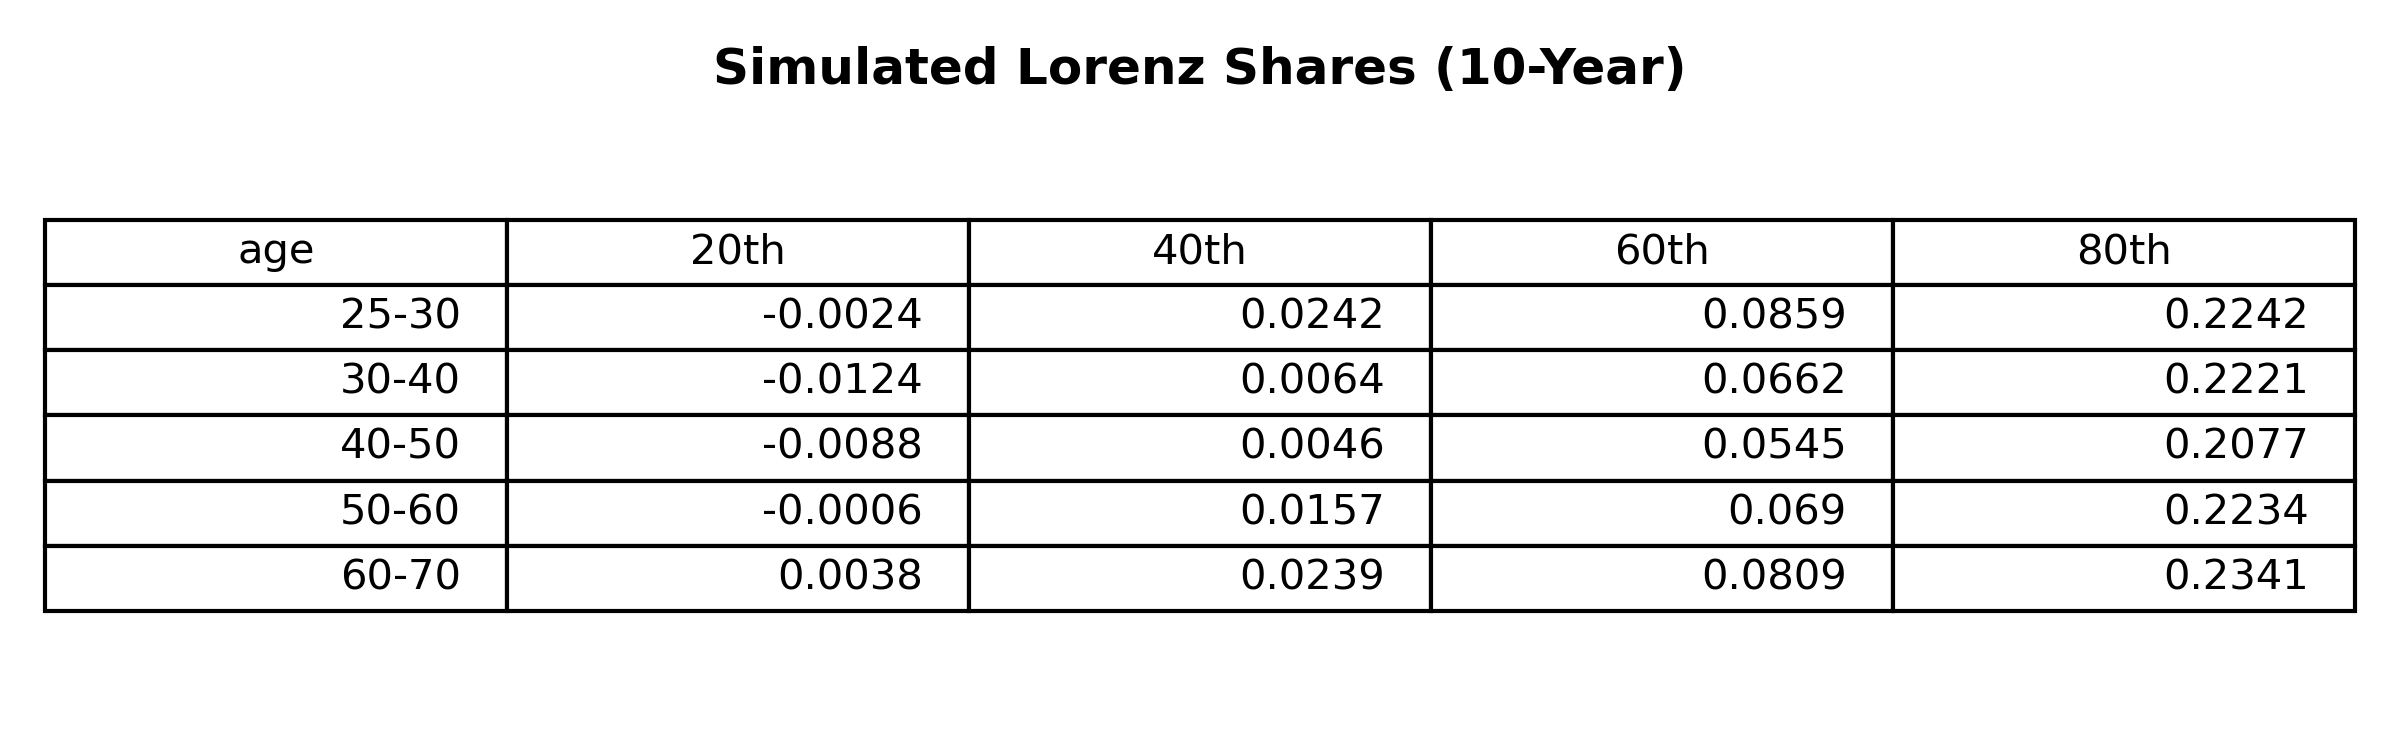
\includegraphics[width=0.8\textwidth]{Tables/Sim_Lorenz_10yr_LCrrDistNetWorth.png}
\caption{Simulated Untargeted Moments with Heterogeneity (R-dist).}
\label{fig:SimLorenzTarDist}
\end{figure}



\par 





